\documentclass{article}
\usepackage[utf8]{inputenc}
\usepackage[T1]{fontenc}
\usepackage{amsmath}
\usepackage{geometry}
\geometry{a4paper, margin=1in}
\usepackage{array} % For controlling table column padding/alignment
\usepackage{multirow} % For multirow command
\usepackage{multicol} % For multicolumn command
\usepackage{tikz} % For drawing the diagram
\usetikzlibrary{shapes, arrows.meta, positioning}
\usepackage{caption} % For figure/table captions

\title{Analysis of Vietnam's Economic Structure}
\date{\today}

\begin{document}
\maketitle

\section{Overview of Economic Sectors}

Vietnam's economy is undergoing a rapid transition, shifting from a predominantly agrarian focus to an industrial and service-oriented structure. This evolution is characterized by strong foreign direct investment (FDI) inflows, particularly into the manufacturing sector, making it a critical component of global supply chains.

A detailed summary of the main economic sectors, including sample data on their estimated contribution to GDP and key characteristics, is provided below. As shown in \textbf{Table~\ref{tab:sectors}}, the Services sector currently accounts for the largest share of GDP, while the Industry sector drives high-value exports and employment growth.

The critical relationship and flow of resources between these three major sectors (Agriculture, Industry, and Services) are crucial for understanding economic resilience and stability. The foundational dependencies and value chain progression are visualized in the organizational chart below. See \textbf{Figure~\ref{fig:flowchart}} for an illustration of the principal inter-sectoral linkages and dependencies.

\subsection{Sectoral Breakdown and Sample Data}

% --- 1. Multirow and Multicolumn Table ---
\begin{table}[h!]
    \centering
    \caption{Summary of Vietnam's Key Economic Sectors (Sample Data)}
    \label{tab:sectors}
    \begin{tabular}{|l|l|c|c|}
        \hline
        \textbf{Sector} & \textbf{Subcategory} & \textbf{Sample GDP \% (Est.)} & \textbf{Workforce \% (Est.)} \\
        \hline
        \multirow{3}{*}{\centering Agriculture}
        & Crops, Forestry & $5.0\%$ & \multirow{3}{*}{\centering $28.0\%$} \\
        \cline{2-3}
        & Livestock, Aquaculture & $3.0\%$ & \\
        \cline{2-3}
        & \multicolumn{2}{|c|}{\textbf{Total Primary Sector Contribution}} & $11.5\%$ (approx) \\
        \hline
        \multirow{2}{*}{\centering Industry}
        & \multicolumn{2}{|c|}{\multirow{2}{*}{\centering Manufacturing (Electronics, Garments)}} & \textbf{$27.5\%$} GDP \\
        \cline{4-4}
        & Construction, Utilities & & $27.0\%$ Workforce \\
        \hline
        \multicolumn{2}{|c|}{\textbf{Services (Trade, Tourism, IT)}} & $45.0\%$ & $45.0\%$ \\
        \hline
    \end{tabular}
\end{table}

\clearpage

\subsection{Inter-sectoral Linkage Diagram}

% --- 2. TikZ Figure ---
\begin{figure}[h!]
    \centering
    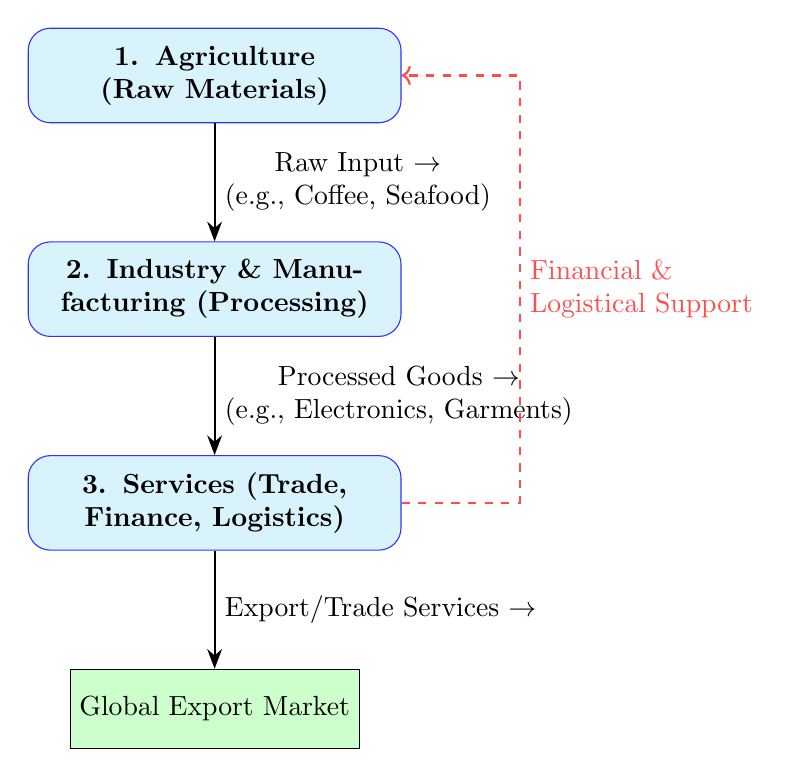
\begin{tikzpicture}[
        block/.style={rectangle, draw=blue!80, fill=cyan!15, text width=4.5cm, text centered, rounded corners=8pt, minimum height=1.2cm, font=\bfseries},
        line/.style={draw, thick, -{Stealth[length=2.5mm]}},
        feedback/.style={draw, thick, dashed, ->, red!70},
        node distance=1.5cm
        ]

        % Nodes
        \node (Agri) [block] {1. Agriculture (Raw Materials)};
        \node (Ind) [block, below=of Agri] {2. Industry \& Manufacturing (Processing)};
        \node (Serv) [block, below=of Ind] {3. Services (Trade, Finance, Logistics)};
        \node (Export) [rectangle, draw, fill=green!20, below=of Serv, minimum height=1cm] {Global Export Market};


        % Arrows
        \draw [line] (Agri.south) -- (Ind.north) node [midway, right, align=center] {Raw Input $\rightarrow$ \\(e.g., Coffee, Seafood)};
        \draw [line] (Ind.south) -- (Serv.north) node [midway, right, align=center] {Processed Goods $\rightarrow$ \\(e.g., Electronics, Garments)};
        \draw [line] (Serv.south) -- (Export.north) node [midway, right, align=center] {Export/Trade Services $\rightarrow$};

        % Feedback Loop / Support
        \draw [feedback] (Serv.east) -- ++(1.5, 0) |- (Agri.east) node [pos=0.25, right, align=left] {Financial \& \\Logistical Support};

    \end{tikzpicture}
    \caption{Inter-sectoral Linkages and Value Chain Flow in Vietnam's Economy}
    \label{fig:flowchart}
\end{figure}

The diagram clearly shows the sequential progression from raw material extraction (Agriculture) to high-value creation (Industry) and finally to market access (Services and Export).
\end{document}
